\section{CMOS}
Most recent update: 2020-04-25 \\
Contact person: Marc Winter (email: marc.winter@iphc.cnrs.fr)

\subsection{Introduction}
CMOS Pixel Sensors (CPS) combine high granularity with low material
budget and allow integrating the full signal processing circuitry on
the sensor substrate. They benefit from a steady technological progress 
driven by an industrial market which makes them simultaneously cost 
effective and attractive for a wide range of applications. They are 
developed for an ILC vertex detector since about two decades and were 
shown to rather easily comply with the required spatial resolution 
and material budget expressed in the DBD~\cite{Behnke:2013lya}. The
associated read-out time of a few tens of microseconds represented the
limit achievable with a rolling shutter read-out and the \SI{350}{\nano\meter} CMOS 
technology available at that time. The required radiation tolerance, 
on the other hand, was observed to be well within the sensor potential.
 
The relevance of the technology for subatomic physics experiments is established today with the 400 ULTIMATE sensors operated in the STAR-PXL 
detector~\cite{CONTIN201860} at RHIC/BNL from 2014 to 2016, while the
state of the art is well illustrated by the $\sim$ 20 times faster ALPIDE sensors fabricated ($>$ 20,000 dies) in a \SI{180}{\nano\meter} CMOS technology, to 
equip the upgraded, $>$ \SI{10}{\meter\squared} large, ALICE Inner Tracker System 
(ITS)~\cite{AGLIERIRINELLA2017583}. 
The variety of devices where ULTIMATE has been implemented and, even 
more so, where ALPIDE is foreseen to be integrated, reflects the maturity 
of the technology and the steadily growing interest it generates in the
field.
 
  The detection performances achieved at the time of the DBD 
assumed that integrating the beam related background over several tens 
of bunch-crossings would result in a well affordable disturbance of the 
event reconstruction. Since then, 
potential benefits from shorter integration times, allowing for bunch 
tagging or nearly so, have become clearer and desirable. This applies 
for instance to the distinction between soft tracks due to beamstrahlung
or two-photon collisions and those originating from a displaced vertex
and therefore contributing to the vertex charge. The latter may get  
particularly complicated to reconstruct in case of a higher machine 
luminosity than foreseen in the TDR and of worse running conditions 
than anticipated. 
  
  However, the goal of suppressing the impact of beam related background 
on the physics performance by improving the sensor time resolution to 
$\lesssim$ \SI{1}{\micro\second} steps up the preexisting tension between the 
small pixel size imposed by the required spatial resolution and the 
minimal space needed to implement the very front end circuitry inside 
the pixels. The R\&D pursued so far did not show that a spatial 
resolution of $\lesssim$ \SI{3}{\micro\meter} and a single bunch tagging are 
actually achievable simultaneously within the same, \SI{50}{\micro\meter} thin, 
sensor with the presently available CMOS technologies, moreover with 
a power consumption compatible with air cooling. On the other hand, 
$\sim$ \SI{4}{\micro\meter} spatial resolution may be within reach with sensors 
featuring a continuous read-out time of $\lesssim$ \SI{1}{\micro\second} at an 
affordable power consumption.

  Indirect approaches are therefore being considered to achieve the 
targeted spatial and time resolutions per layer even if they cannot be
reached within a single sensor. They rely on the concept of double-sided detector layers, which provides two hits, one per layer face, for each traversing charged particle. The track 
position and timing are extracted from the combination of the two 
signals delivered by sensors facing each other in the same layer. 
The position and timing may, for instance, come from a high precision 
sensor located on one layer side and a faster, less precise, sensor 
located on the opposite side. Alternatively, the spatial resolution 
may be derived from the combination of opposite, identical, sensors 
limited to \SI{4}{\micro\meter} spatial resolution measurements but providing 
both $\lesssim$ \SI{1}{\micro\second} read-out time.     

\begin{figure}
	\centering
	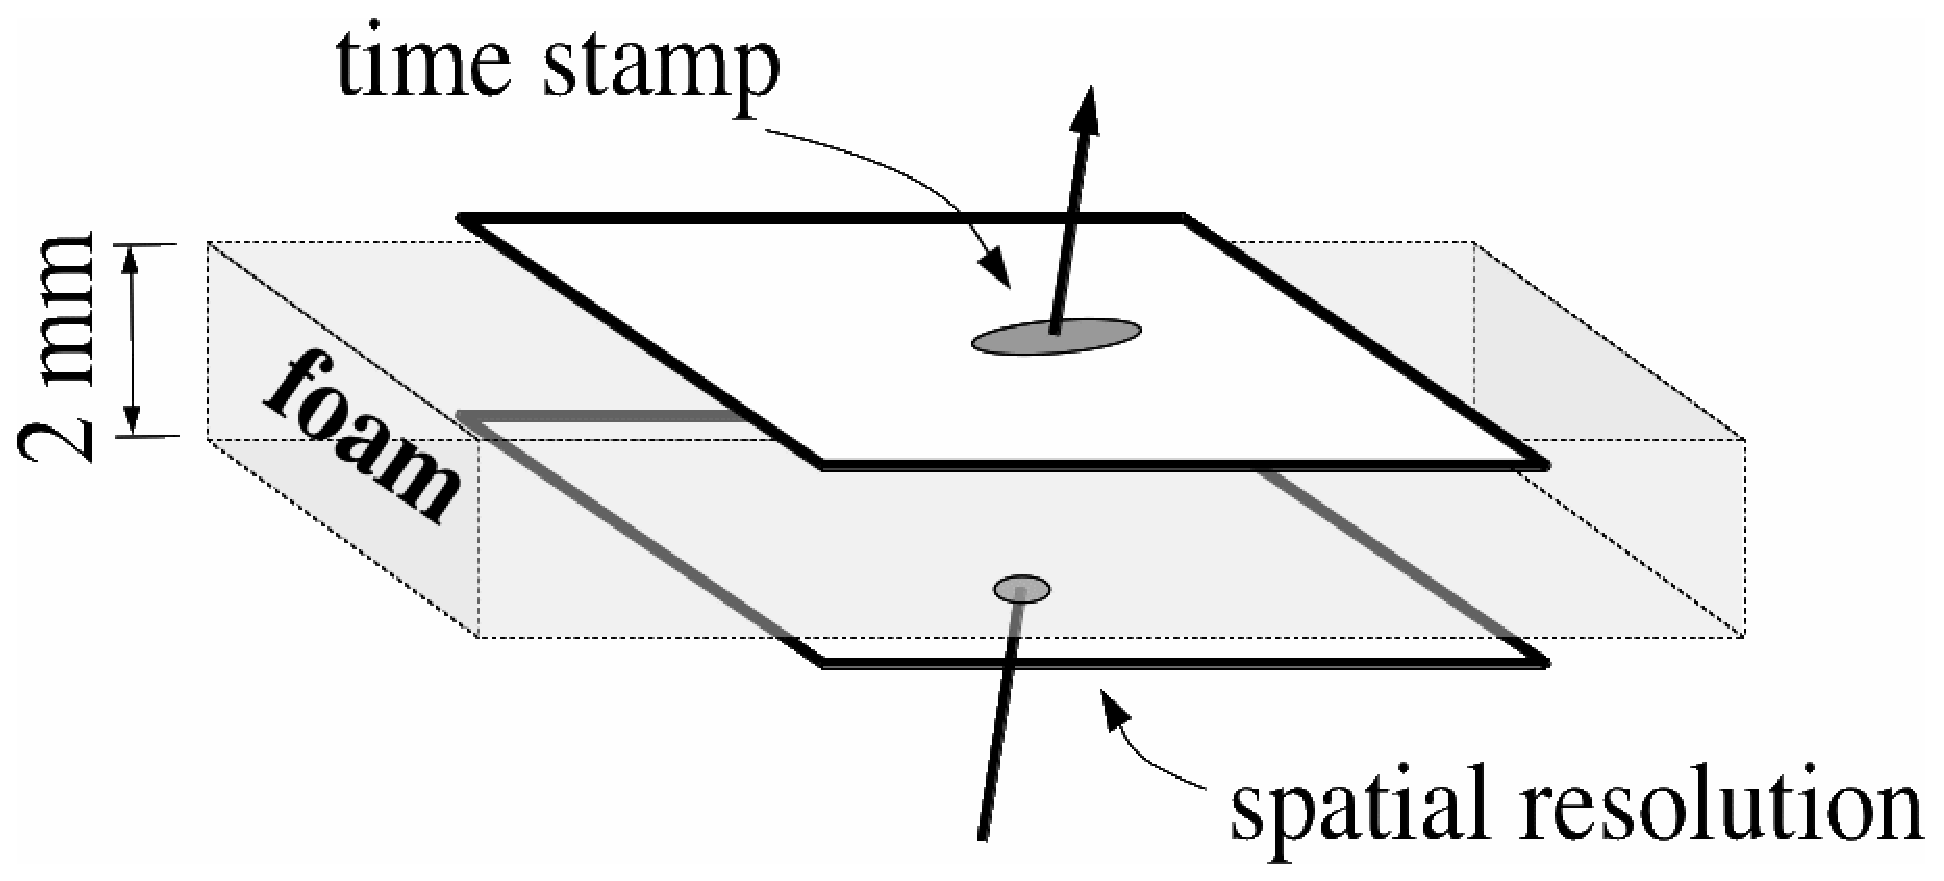
\includegraphics[width=.43\linewidth]{VertexDetector/CMOS/principe-MixedLayers-noPixels.eps}
	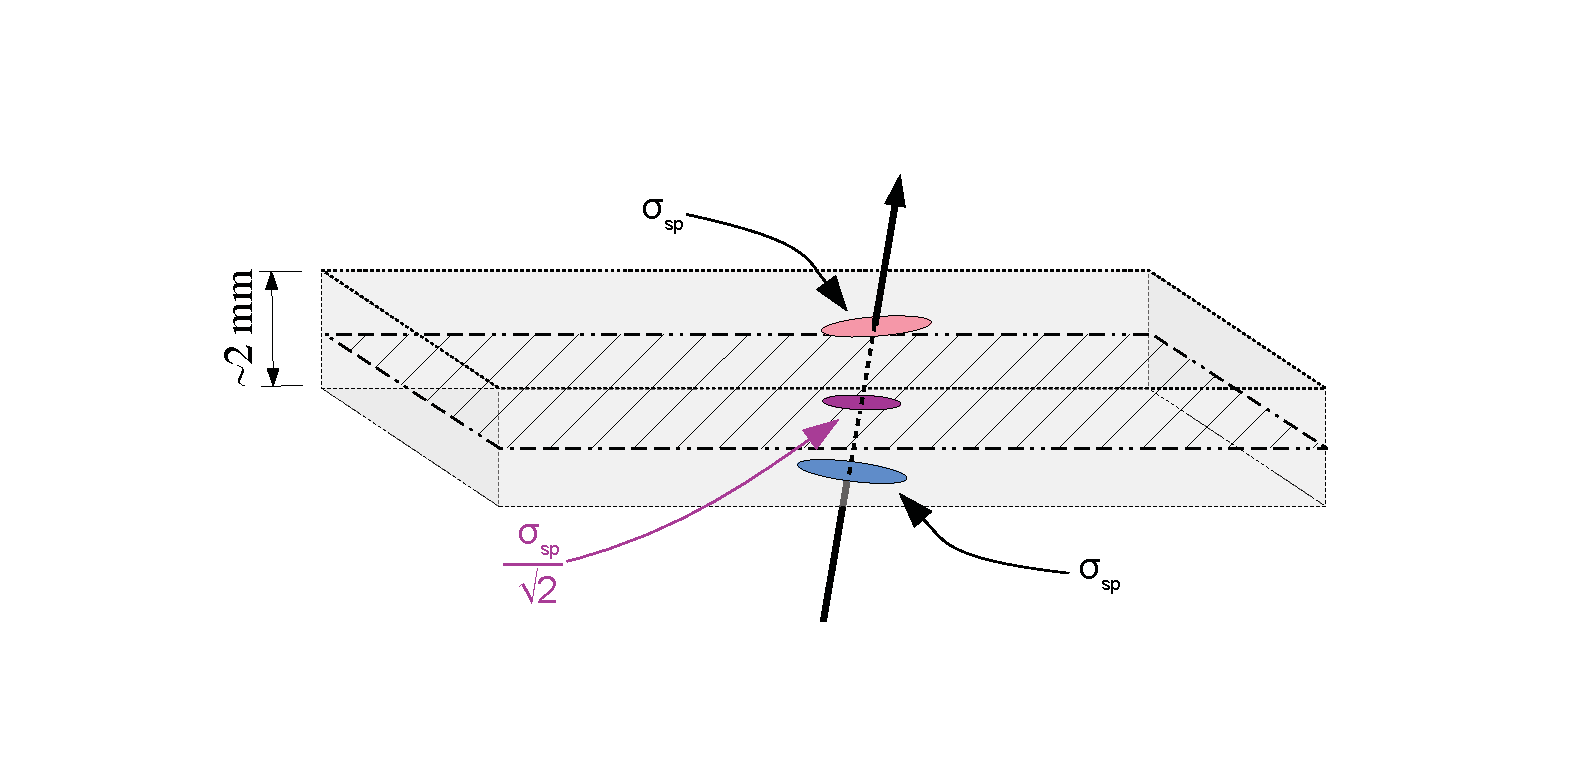
\includegraphics[width=.55\linewidth]{VertexDetector/CMOS/principe-MixedLayers-intermediatePoint.pdf}
	\caption{Alternative approaches based on double-sided layers. Left: particles traverse a "pointing" sensor and a ``timing'' sensor equipping the two faces of a layer. Right: the signals of two ``timing'' sensors featuring $\sim$ \SI{4}{\micro\meter} resolution are combined into a single signal to obtain the required spatial resolution of $\lesssim$ \SI{3}{\micro\meter}.}
	\label{fig:VertexDetector:CMOS:minivectors}
\end{figure}

\subsection{Recent Milestones}
The most advanced CPS under development extendable to bridge the 
gap between ALPIDE and a sensor adapted to an ILC vertex detector 
is the MIMOSIS sensor~\cite{Morel:mimosis}, which is foreseen to 
equip the 4 double-sided stations of the MicroVertex Detector (MVD) 
of the CBM heavy ion experiment at FAIR/GSI. The sensor acts 
simultaneously as a forerunner of a sensor suited to an ILC vertex 
detector. With a pixel array continuous read-out derived from ALPIDE, 
MIMOSIS features a 50 times higher hit density treatment capability 
and a \SI{5}{\micro\second} read-out time. The latter may be compressed to 
$\sim$ \SI{2}{\micro\second} for an ILC vertex detector, with an instantaneous 
power density in the order of $\sim$ \SIrange{50}{150}{\milli\watt\per\centi\meter\squared}, depending 
on the beam background induced hit density, and thereby on the 
distance to the interaction point. Such performances should allow 
facing the most pessimistic predictions for the background rate 
impinging the vertex detector innermost layer. 

The sensor single point resolution however, is not expected to reach
values well below the ALPIDE value of \SI{5}{\micro\meter} because of the pixel 
footprint imposed by the required in-pixel circuitry, which involves 
about 200 transistors. Optimizing the spatial resolution will consist 
in enhancing charge sharing by using the most appropriate epitaxial 
layer thickness and by tuning the depletion voltage and the steering 
parameters of the in-pixel circuitry. 

After a first prototyping step validating the in-pixel circuitry and the 
pixel array read-out (prototype MIMOSIS-0 featuring $64 \times 504$ pixels), 
the first full scale prototype of MIMOSIS has been fabricated. It 
incorporates $1024 \times 504$ pixels of $\SI{27}{\micro\meter} \times \SI{30}{\micro\meter}$. Its manufacturing 
was accompanied by numerous small prototypes exploring in-pixel circuitry alternatives, allowing in particular for shorter read-out time. They 
are supposed to complement studies made with MIMOSIS-0 showing that the 
sensor charge collection system and the very front-end circuitry are 
suited read-out times shorter than \SI{1}{\micro\second}~\cite{DEVEAUX2020162653}. 
The performance assessment of the complete read-out chain should come 
out through year 2021. Besides the vertex detector, this R\&D also 
applies to tracking subsystems in general. An emblematic example is 
the ILD-SIT, which may be equipped with double-sided layers based on 
$\gtrsim$ \SI{5}{\micro\meter} resolution CPS featuring \SI{1}{\micro\second} read-out time.

 \begin{figure}
	\centering
	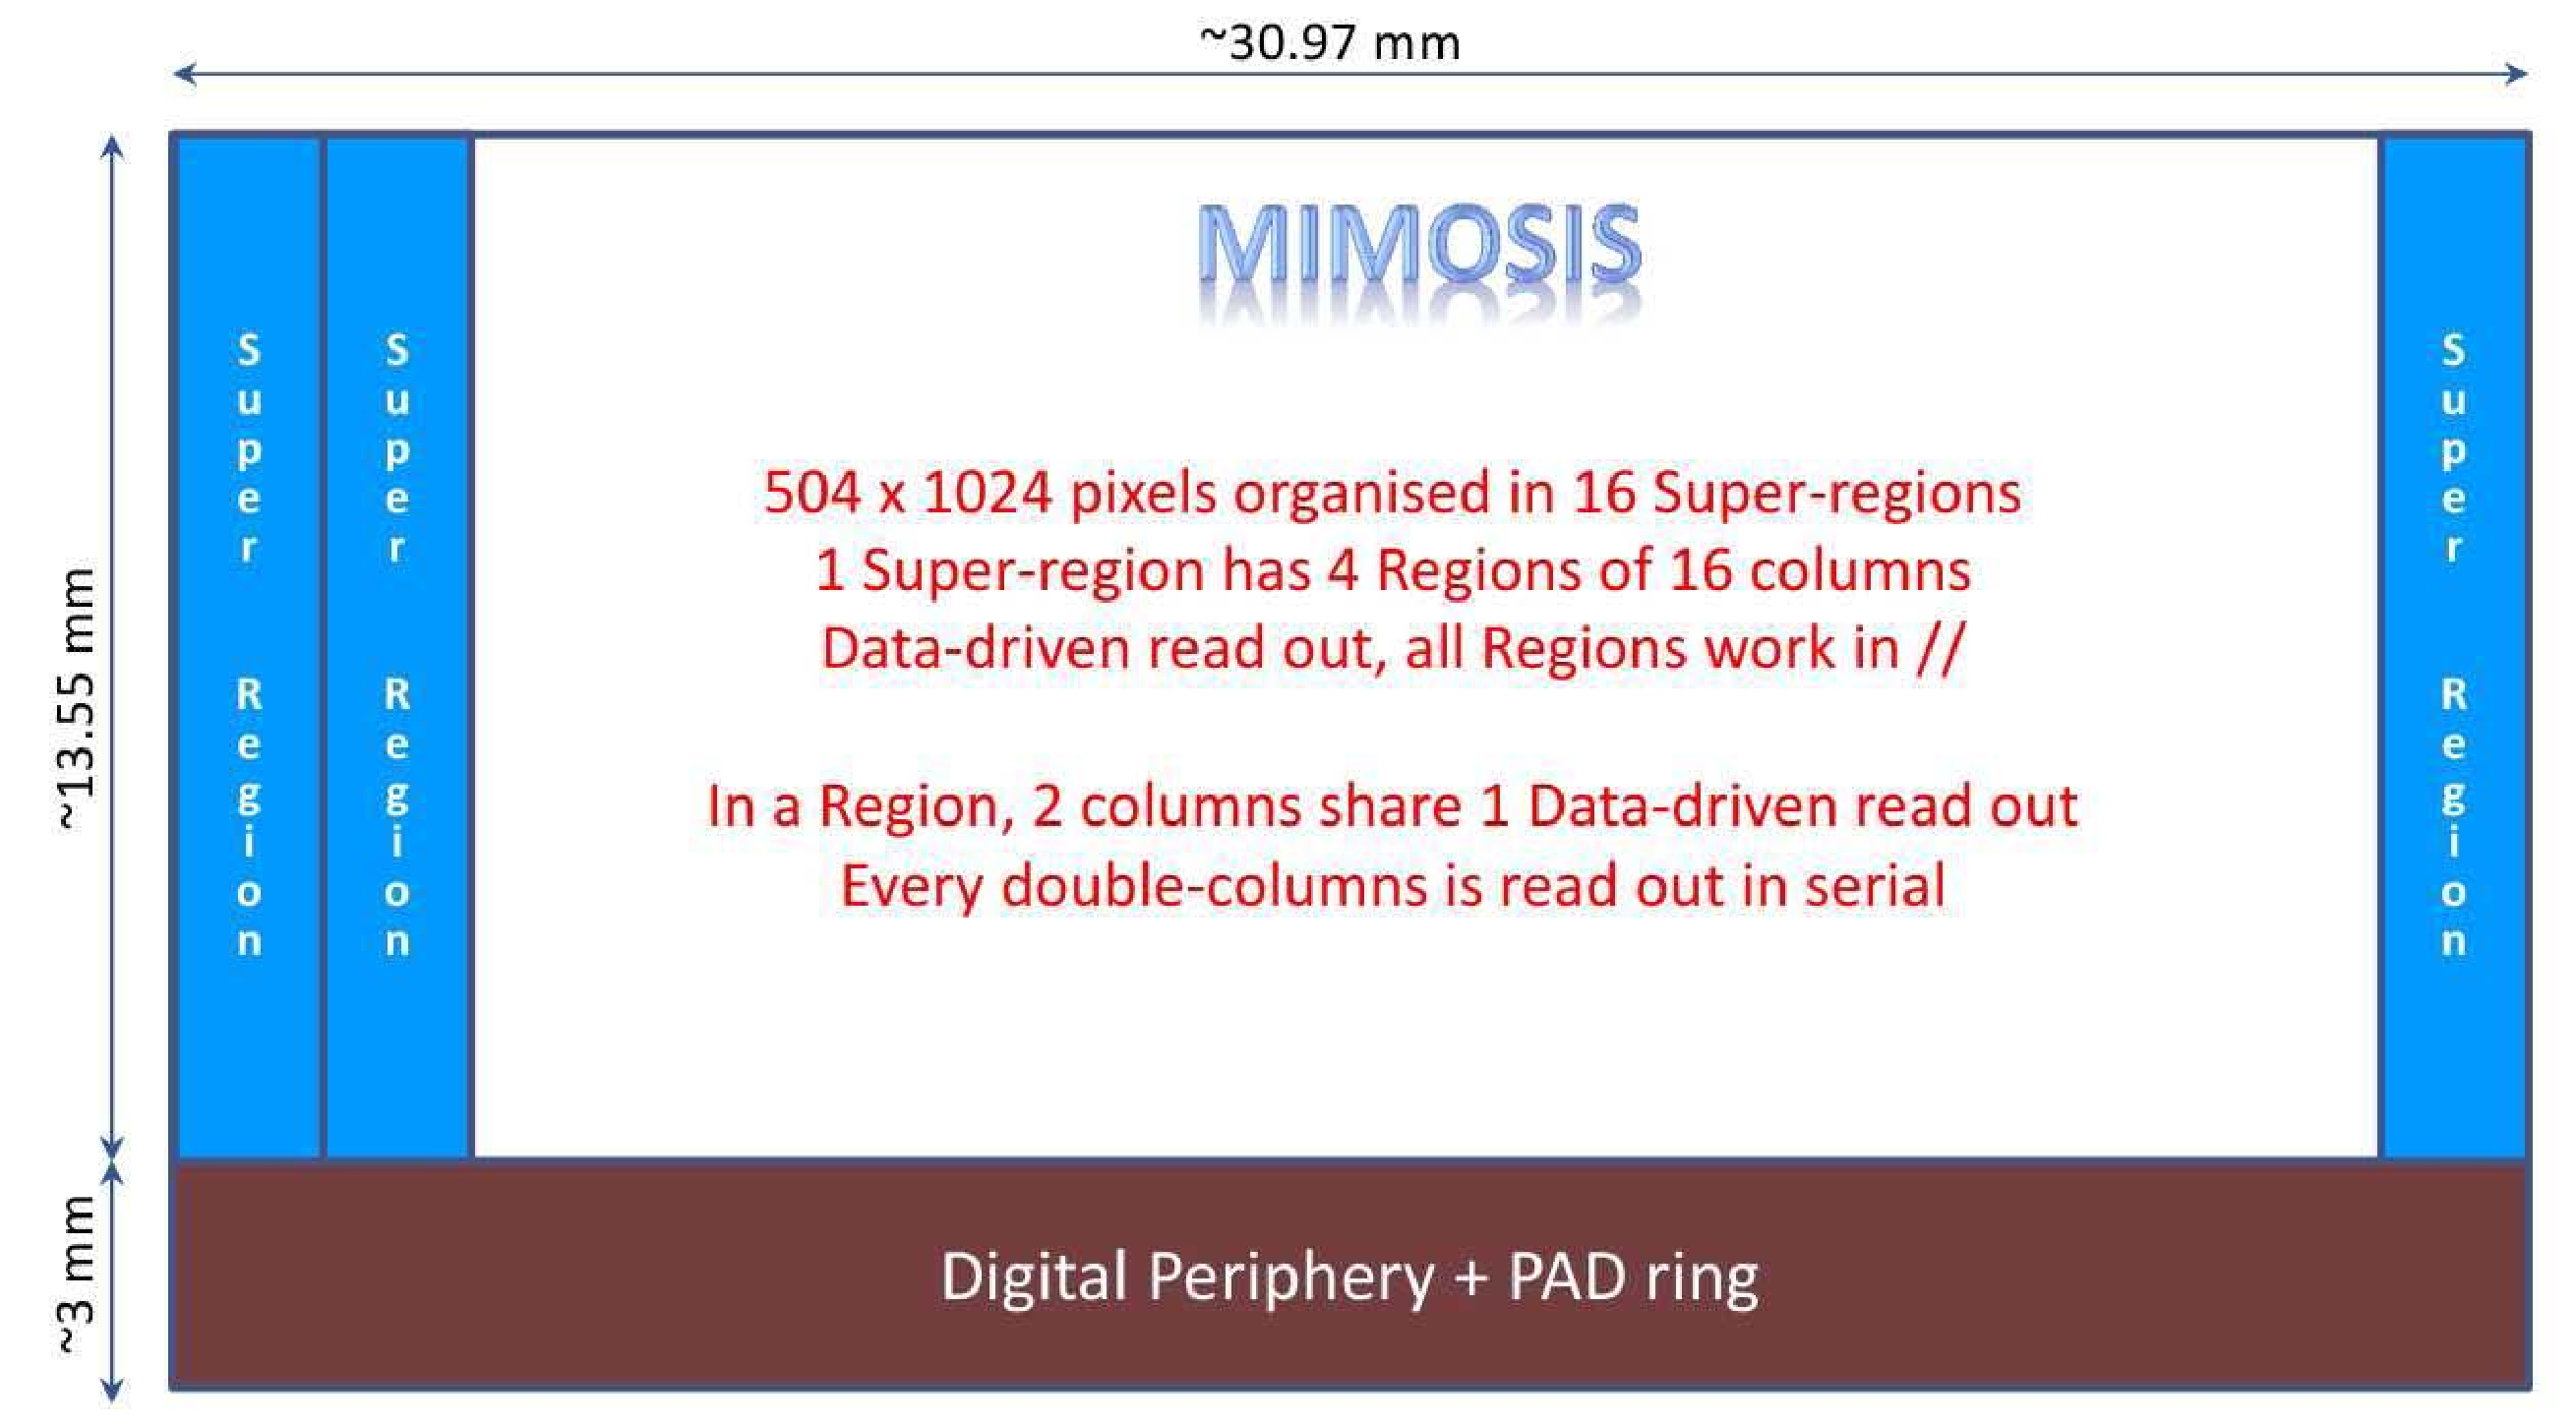
\includegraphics[width=.7\linewidth]{VertexDetector/CMOS/CHG-slide4.pdf}
	\caption{Schematic representation of the MIMOSIS sensor developed to equip the CBM-MVD.}
	\label{fig:VertexDetector:CMOS:MIMOSIS}
\end{figure}
\begin{figure}
	\centering
	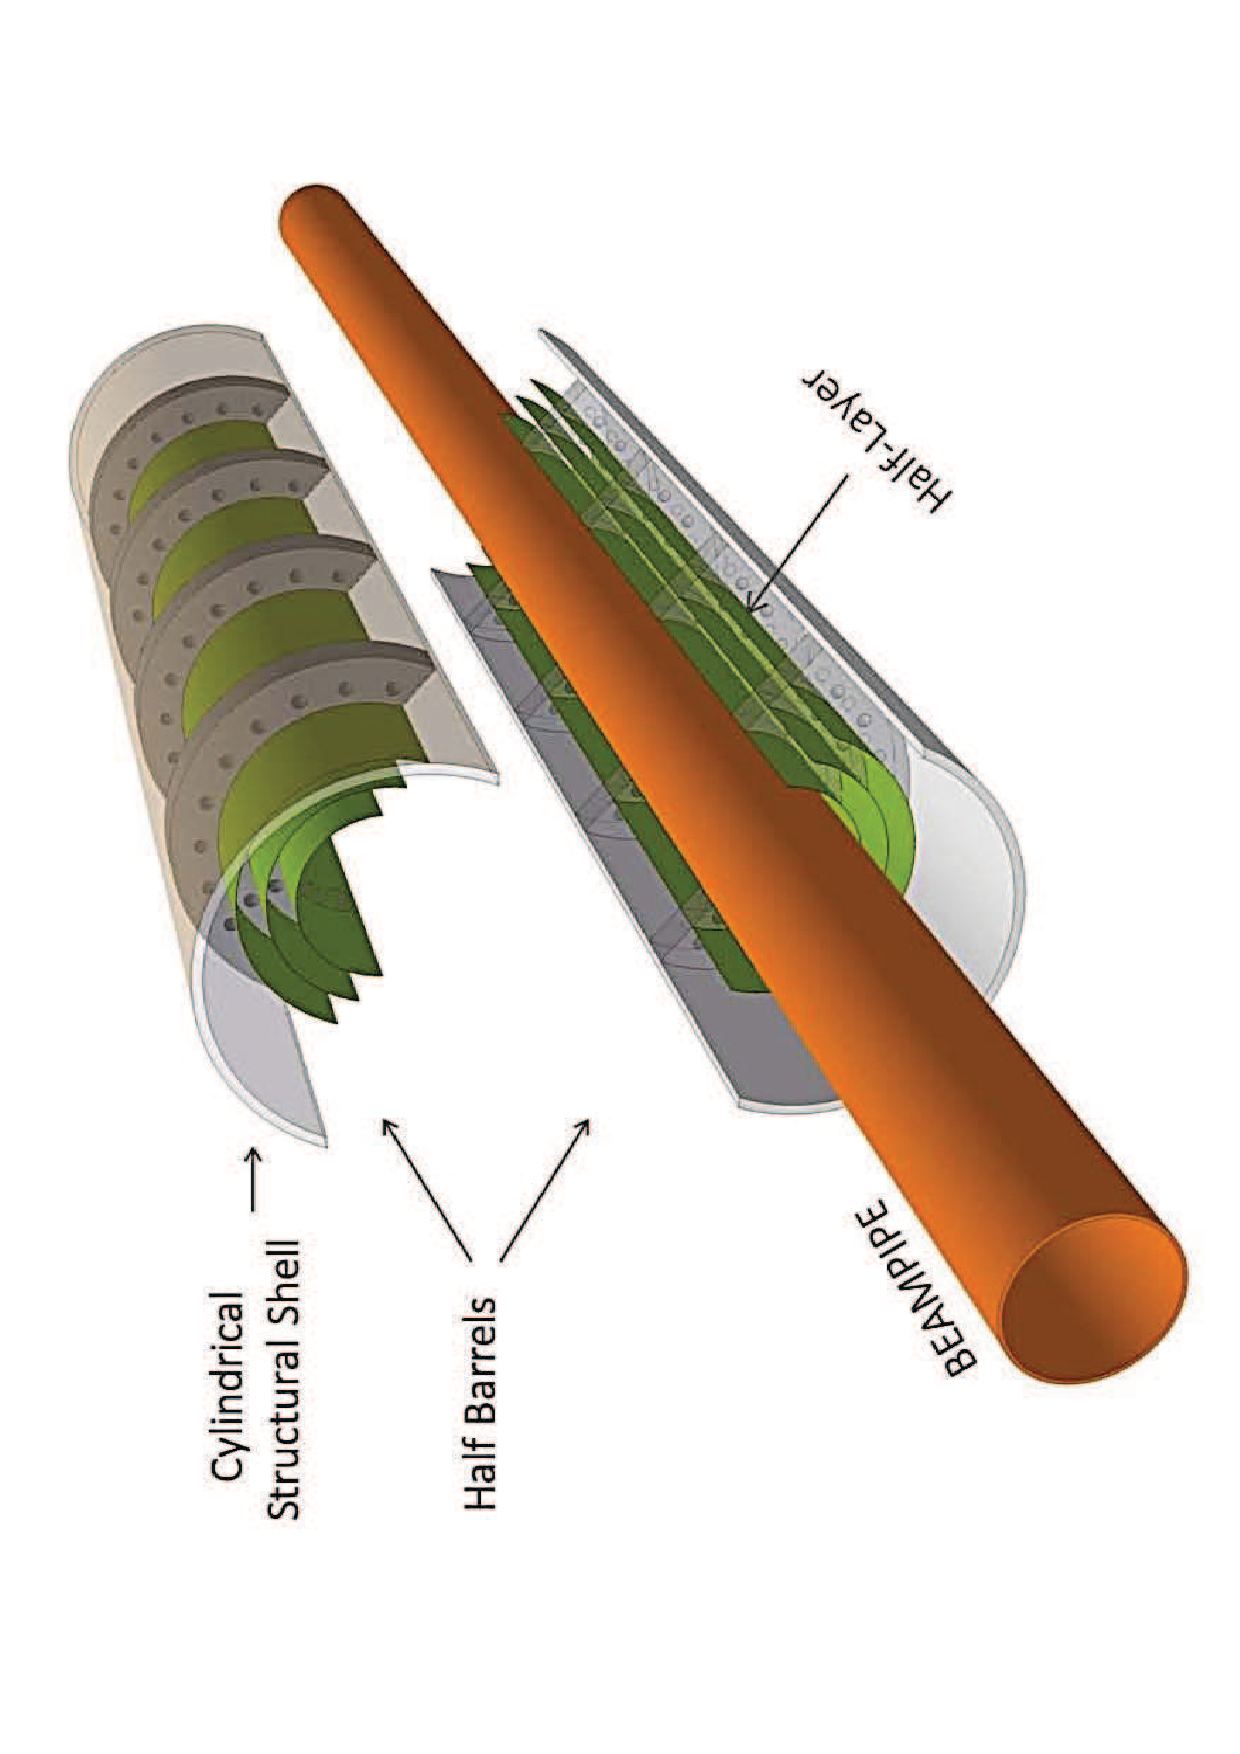
\includegraphics[angle=270, width=.5\linewidth]{VertexDetector/CMOS/ALICE-Vertex-Stitched.pdf}
    \caption{Schematic view illustrating the concept of a vertex detector based on stitched sensors curved according to a cylindrical geometry.}
	\label{fig:VertexDetector:CMOS:stitching}
\end{figure}

Another important step achieved in recent years is the first operation 
of ultra-light double-sided pixelated ladders in a real experimental 
environment, based on two PLUME devices installed near the interaction 
region of the BELLE-II experiment during the beam commissioning phase 
called BEAST-II~\cite{CUESTA2020163862}. The ladders were ran successfully 
through the period, contributing to the monitoring of the background 
induced by SuperKEKB in the inner tracker volume with their \SI{3.3}{\micro\meter}
single point resolution and their low material budget ($\sim$ \mbox{0.4\% X$_0$}),
despite their modest read-out speed (\SI{115}{\micro\second}).   


Squeezing the material budget of the double-sided PLUME ladders to 
$\lesssim~0.3\%~X_0$ remains of prime interest but represents a major engineering challenge, possibly complicated by the necessity to 
power pulse ladders in the strong experimental magnetic field. 
Power pulsing is suspected to be needed in case of continuous 
read-out with the present sensor design, derived from MIMOSIS. 
However, whether it will be needed for all layers and for a sensor
fabrication process with smaller feature size remains an open 
question. Moreover, the possibility to introduce micro-channel 
cooling in the ladders will also be considered in order to mitigate 
power pulsing requirements.

Another engineering challenge may follow from the possibility 
to realise wafer scale sensors benefitting from the stitching
proposed by CMOS foundries for commercial imagers (see the next
subsection). In this case, the sensors would be curved to form 
large parts of a cylinder and would need a specific mechanical
concept to ensure rigidity and low mass cooling services.  

\subsection{Future Plans}
The achieved performances, which may already be considered as 
relatively satisfactory, are anticipated to be boosted in the 
coming years by industrial progress, following in particular 
from evolutions of the ASIC production technology, which drives 
steady miniaturization of integrated circuits. CMOS foundries 
also offer the possibility of stitching, which allows for 
wafer-scale sensors. Once thinned to a few tens of microns, 
the sensor may be curved according to a cylindrical surface, 
with a sizeable gain in stiffness. A few sensors only are then 
required to equip a complete detector layer, with a drastic 
suppression of mechanical support material consecutive to the 
disappearance of overlaps between neighboring detector modules. 
This concept is promoted by the ALICE collaboration, which aims 
for an upgrade of its vertex detector~\cite{CERN-LHCC-2019-018}. Maximum 
benefit is expected for the innermost detector layer, where the 
beam pipe may act as a mechanical support. 

  Stitching is available in the \SI{180}{\nano\meter} CMOS process used for 
ALPIDE and MIMOSIS. It is also accessible in a forthcoming 65~nm 
imaging process investigated at CERN within a partnership involving 
groups interested in various applications, including ILC related 
tracking devices. The process should in particular allow for 
reduced pixel dimensions, and therefore improved single point 
resolution. Overall, the evolution toward this \SI{65}{\nano\meter} CMOS process 
is particularly appealing and should take advantage from a 
cross-fertilization between numerous projects.

  Another promising R\&D direction addresses the realization of 
two-tier chips interconnected at the pixel level through industrial 
micro-bonding techniques. High-density micro-bonding is getting 
widespread, which allows to distribute the analog front-end and 
the digital circuitry of a pixel among two different chips being 
ultimately interconnected at the pixel level. The result is a 
reduced pixel size which improves the spatial resolution and 
enhances the data compression. A micro-bonding process already 
successfully tried with SoI sensors, is getting explored with CPS.
